% Options for packages loaded elsewhere
\PassOptionsToPackage{unicode}{hyperref}
\PassOptionsToPackage{hyphens}{url}
%
\documentclass[
]{article}
\usepackage{lmodern}
\usepackage{amsmath}
\usepackage{ifxetex,ifluatex}
\ifnum 0\ifxetex 1\fi\ifluatex 1\fi=0 % if pdftex
  \usepackage[T1]{fontenc}
  \usepackage[utf8]{inputenc}
  \usepackage{textcomp} % provide euro and other symbols
  \usepackage{amssymb}
\else % if luatex or xetex
  \usepackage{unicode-math}
  \defaultfontfeatures{Scale=MatchLowercase}
  \defaultfontfeatures[\rmfamily]{Ligatures=TeX,Scale=1}
  \setmainfont[]{Arial}
\fi
% Use upquote if available, for straight quotes in verbatim environments
\IfFileExists{upquote.sty}{\usepackage{upquote}}{}
\IfFileExists{microtype.sty}{% use microtype if available
  \usepackage[]{microtype}
  \UseMicrotypeSet[protrusion]{basicmath} % disable protrusion for tt fonts
}{}
\makeatletter
\@ifundefined{KOMAClassName}{% if non-KOMA class
  \IfFileExists{parskip.sty}{%
    \usepackage{parskip}
  }{% else
    \setlength{\parindent}{0pt}
    \setlength{\parskip}{6pt plus 2pt minus 1pt}}
}{% if KOMA class
  \KOMAoptions{parskip=half}}
\makeatother
\usepackage{xcolor}
\IfFileExists{xurl.sty}{\usepackage{xurl}}{} % add URL line breaks if available
\IfFileExists{bookmark.sty}{\usepackage{bookmark}}{\usepackage{hyperref}}
\hypersetup{
  pdftitle={Problem Set 01: Intro to R and RStudio},
  hidelinks,
  pdfcreator={LaTeX via pandoc}}
\urlstyle{same} % disable monospaced font for URLs
\usepackage[margin=1in]{geometry}
\usepackage{color}
\usepackage{fancyvrb}
\newcommand{\VerbBar}{|}
\newcommand{\VERB}{\Verb[commandchars=\\\{\}]}
\DefineVerbatimEnvironment{Highlighting}{Verbatim}{commandchars=\\\{\}}
% Add ',fontsize=\small' for more characters per line
\usepackage{framed}
\definecolor{shadecolor}{RGB}{248,248,248}
\newenvironment{Shaded}{\begin{snugshade}}{\end{snugshade}}
\newcommand{\AlertTok}[1]{\textcolor[rgb]{0.94,0.16,0.16}{#1}}
\newcommand{\AnnotationTok}[1]{\textcolor[rgb]{0.56,0.35,0.01}{\textbf{\textit{#1}}}}
\newcommand{\AttributeTok}[1]{\textcolor[rgb]{0.77,0.63,0.00}{#1}}
\newcommand{\BaseNTok}[1]{\textcolor[rgb]{0.00,0.00,0.81}{#1}}
\newcommand{\BuiltInTok}[1]{#1}
\newcommand{\CharTok}[1]{\textcolor[rgb]{0.31,0.60,0.02}{#1}}
\newcommand{\CommentTok}[1]{\textcolor[rgb]{0.56,0.35,0.01}{\textit{#1}}}
\newcommand{\CommentVarTok}[1]{\textcolor[rgb]{0.56,0.35,0.01}{\textbf{\textit{#1}}}}
\newcommand{\ConstantTok}[1]{\textcolor[rgb]{0.00,0.00,0.00}{#1}}
\newcommand{\ControlFlowTok}[1]{\textcolor[rgb]{0.13,0.29,0.53}{\textbf{#1}}}
\newcommand{\DataTypeTok}[1]{\textcolor[rgb]{0.13,0.29,0.53}{#1}}
\newcommand{\DecValTok}[1]{\textcolor[rgb]{0.00,0.00,0.81}{#1}}
\newcommand{\DocumentationTok}[1]{\textcolor[rgb]{0.56,0.35,0.01}{\textbf{\textit{#1}}}}
\newcommand{\ErrorTok}[1]{\textcolor[rgb]{0.64,0.00,0.00}{\textbf{#1}}}
\newcommand{\ExtensionTok}[1]{#1}
\newcommand{\FloatTok}[1]{\textcolor[rgb]{0.00,0.00,0.81}{#1}}
\newcommand{\FunctionTok}[1]{\textcolor[rgb]{0.00,0.00,0.00}{#1}}
\newcommand{\ImportTok}[1]{#1}
\newcommand{\InformationTok}[1]{\textcolor[rgb]{0.56,0.35,0.01}{\textbf{\textit{#1}}}}
\newcommand{\KeywordTok}[1]{\textcolor[rgb]{0.13,0.29,0.53}{\textbf{#1}}}
\newcommand{\NormalTok}[1]{#1}
\newcommand{\OperatorTok}[1]{\textcolor[rgb]{0.81,0.36,0.00}{\textbf{#1}}}
\newcommand{\OtherTok}[1]{\textcolor[rgb]{0.56,0.35,0.01}{#1}}
\newcommand{\PreprocessorTok}[1]{\textcolor[rgb]{0.56,0.35,0.01}{\textit{#1}}}
\newcommand{\RegionMarkerTok}[1]{#1}
\newcommand{\SpecialCharTok}[1]{\textcolor[rgb]{0.00,0.00,0.00}{#1}}
\newcommand{\SpecialStringTok}[1]{\textcolor[rgb]{0.31,0.60,0.02}{#1}}
\newcommand{\StringTok}[1]{\textcolor[rgb]{0.31,0.60,0.02}{#1}}
\newcommand{\VariableTok}[1]{\textcolor[rgb]{0.00,0.00,0.00}{#1}}
\newcommand{\VerbatimStringTok}[1]{\textcolor[rgb]{0.31,0.60,0.02}{#1}}
\newcommand{\WarningTok}[1]{\textcolor[rgb]{0.56,0.35,0.01}{\textbf{\textit{#1}}}}
\usepackage{graphicx}
\makeatletter
\def\maxwidth{\ifdim\Gin@nat@width>\linewidth\linewidth\else\Gin@nat@width\fi}
\def\maxheight{\ifdim\Gin@nat@height>\textheight\textheight\else\Gin@nat@height\fi}
\makeatother
% Scale images if necessary, so that they will not overflow the page
% margins by default, and it is still possible to overwrite the defaults
% using explicit options in \includegraphics[width, height, ...]{}
\setkeys{Gin}{width=\maxwidth,height=\maxheight,keepaspectratio}
% Set default figure placement to htbp
\makeatletter
\def\fps@figure{htbp}
\makeatother
\setlength{\emergencystretch}{3em} % prevent overfull lines
\providecommand{\tightlist}{%
  \setlength{\itemsep}{0pt}\setlength{\parskip}{0pt}}
\setcounter{secnumdepth}{-\maxdimen} % remove section numbering
\ifluatex
  \usepackage{selnolig}  % disable illegal ligatures
\fi

\title{Problem Set 01: Intro to R and RStudio}
\author{}
\date{\vspace{-2.5em}}

\begin{document}
\maketitle

{
\setcounter{tocdepth}{2}
\tableofcontents
}
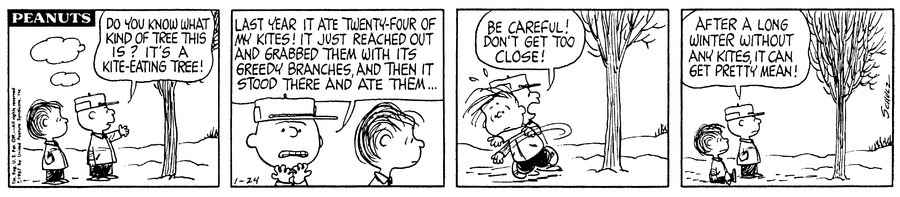
\includegraphics[width=1\textwidth,height=\textheight]{figures/cbrown.jpg}

The goal this week is to introduce you to R and RStudio which you'll be
using throughout the course both to review the statistical concepts
discussed in the course and to analyze real data and come to informed
conclusions. To clarify which is which: R is the name of the programming
language itself and RStudio is a convenient interface.

Today we begin with the fundamental building blocks of R and RStudio:
the interface, creating and saving files, and basic commands.

\hypertarget{the-rstudio-interface}{%
\section{The RStudio Interface}\label{the-rstudio-interface}}

In RStudio you should see a window that looks like the image below.

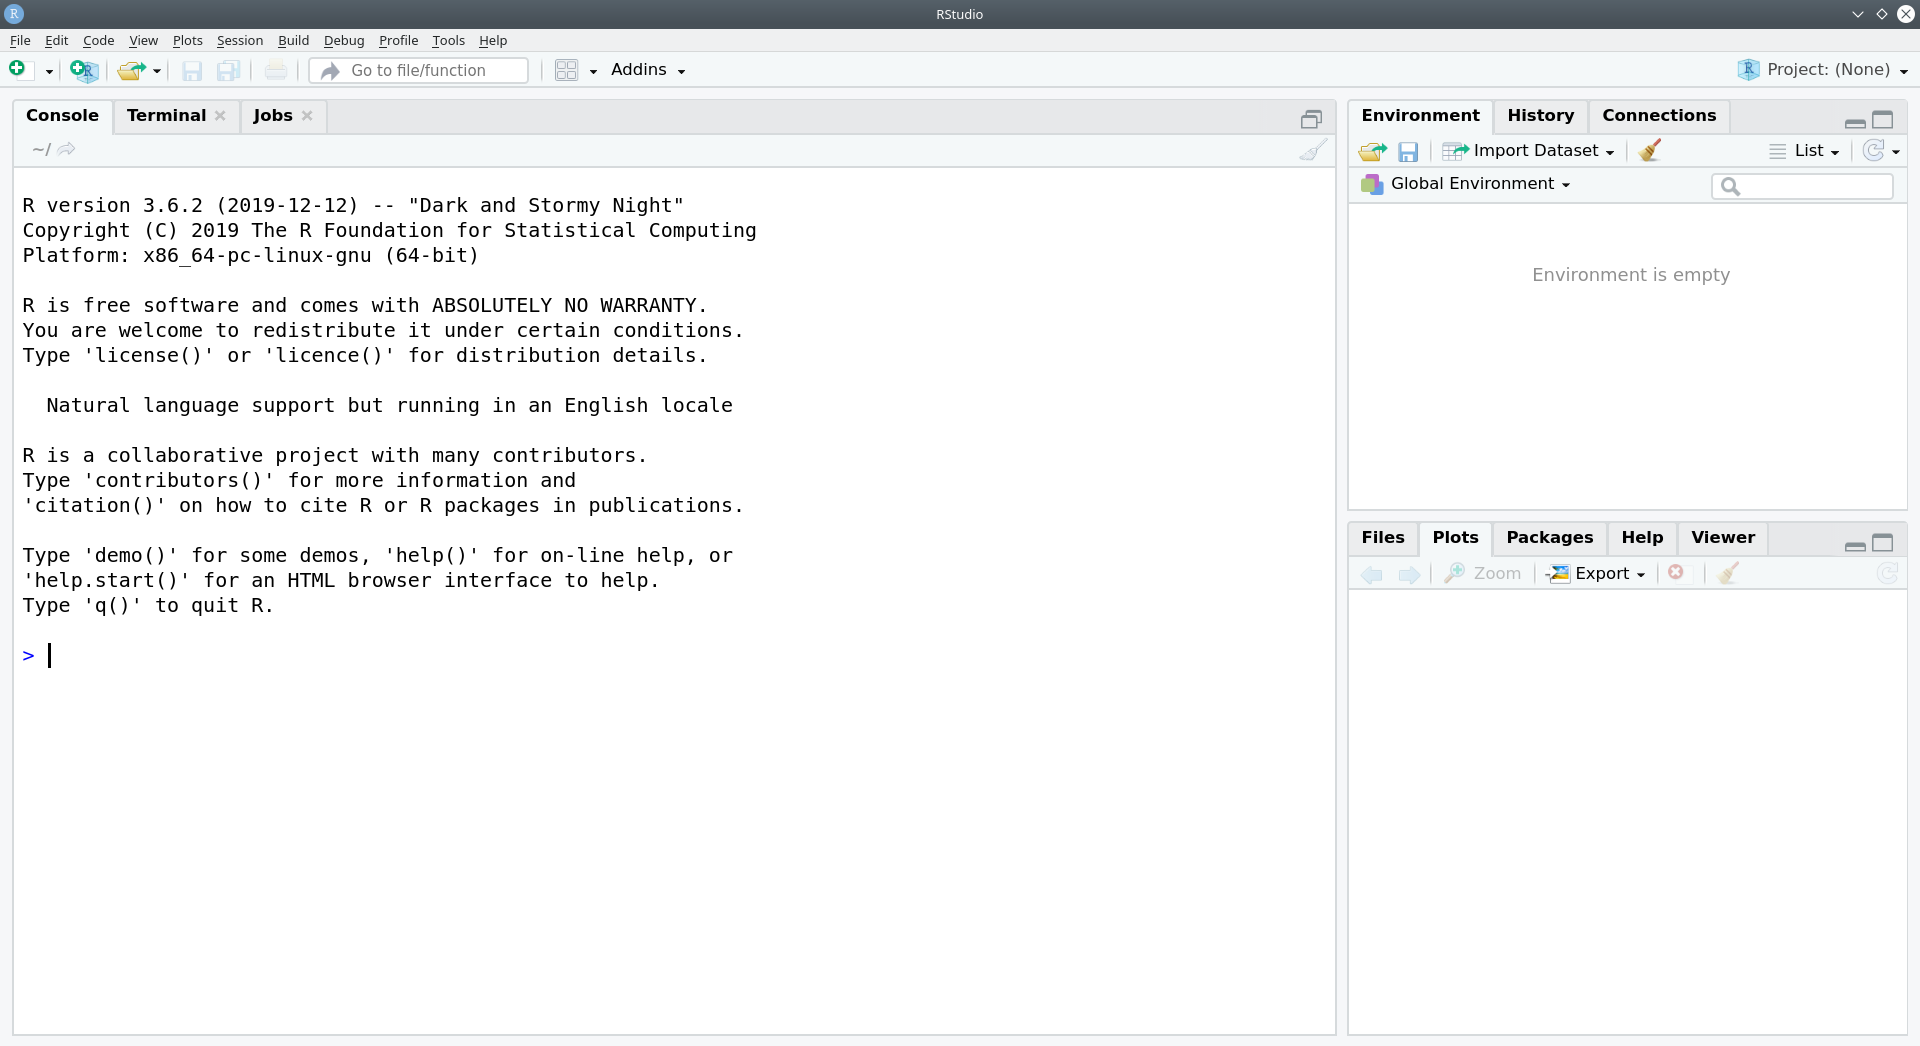
\includegraphics[width=1\textwidth,height=\textheight]{figures/Studio_desktop_opening.png}

The panel on the left is where the action happens. It's called the
\emph{console}. Every time you launch RStudio, it will have the same
text at the top of the console telling you the version of R that you're
running.

The panel in the upper right contains your \emph{workspace}. This shows
the variables and objects you define during your R session, and a
history of the commands that you enter.

Any plots that you generate will show up in the panel in the lower right
corner. This is also where you can browse your files, and access help
files, and upload and download files.

\hypertarget{using-r-markdown-files}{%
\section{Using R Markdown files}\label{using-r-markdown-files}}

\hypertarget{opening-a-new-file}{%
\subsection{Opening a new file}\label{opening-a-new-file}}

When you want to write a paper, you have to open a Word document to type
your ideas into, and save your work in. In R we use a document type
called an R Markdown document. R Markdown documents are useful for both
running code, and annotating the code with comments. The document can be
saved, so you can refer back to your code later, and can be used to
create other document types (html, word, pdf, or slides) for presenting
the results of your analyses. R Markdown provides a way to generate
clear and reproducible statistical analyses.

To open a new file, click on the little green plus on the upper left
hand, and select R Markdown, as in the image below. You can leave it
untitled.

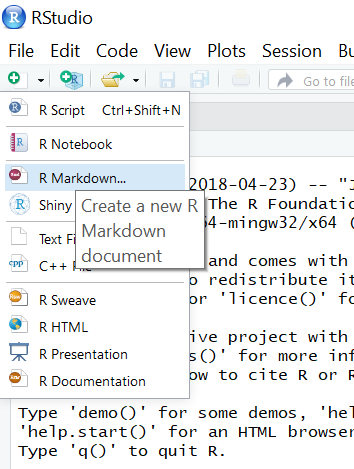
\includegraphics[width=2.60417in,height=\textheight]{figures/how.to.open.rmd.png}

When you open a new R Markdown file, there is some example code in it
that you can get rid of. We will take care of this next.

\hypertarget{make-changes-to-a-file}{%
\subsection{Make changes to a file}\label{make-changes-to-a-file}}

Let's make some changes to the R Markdown file you just opened. Using
the image below as a guide

\begin{itemize}
\tightlist
\item
  First, change the title of the lab at the top to ``Getting to know
  RStudio''. Be sure to keep the quotation marks.
\item
  Second, add an author line, following the example below. You need
  quotation marks!
\item
  Third, delete everything in the document from line 6 downwards.
\item
  Fourth, add headers and text, \textbf{exactly} following the example
  below.
\item
  Finally, insert what is called a ``code chunk.'' To do this you click
  on the \textbf{insert} button near the top center of the screen, then
  choose R. The greyed out box that shows up is where you type code.
\end{itemize}

Your final result should look like this:

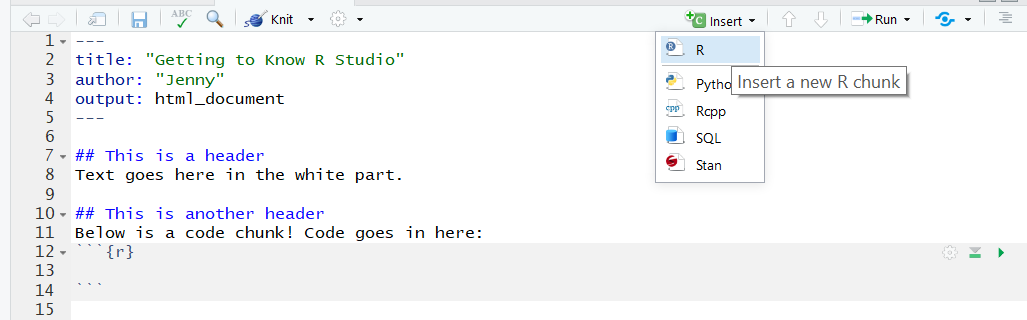
\includegraphics[width=1\textwidth,height=\textheight]{figures/make.changes.png}

\hypertarget{saving-a-file}{%
\subsection{Saving a file}\label{saving-a-file}}

You will complete your lab work in an R Markdown file like this each
week, so it is important to learn how to save these files.

\begin{itemize}
\tightlist
\item
  Click File \textgreater{} Save As\ldots{}
\item
  Browse to the folder where you want to store the R Markdown document
  and it's output.
\item
  Name the file something informative, e.g.,
  \texttt{PS01\_lastname\_firstname} (fill in your first name and last
  name). Make sure to keep the \texttt{.Rmd} file extension.
\item
  Click save
\end{itemize}

\leavevmode\hypertarget{license}{}%
Keeping track of how you organize your folders and files, and being
consistent, will help save you \textbf{a lot} of headaches as you start
coding in R. It would be a good idea to create a folder where you store
all your problem sets, or create one folder for each problem set. Either
way, be consistent and pay attention to your organization.

\hypertarget{knitting-an-html-file}{%
\subsection{Knitting an HTML file}\label{knitting-an-html-file}}

Click the Knit button at the top left side of the screen to ``knit'' the
file, or in other words, produce an output document. An \texttt{.html}
file will be generated. It is automatically saved in the same folder
that your R Markdown file was saved in.

\leavevmode\hypertarget{license}{}%
If you see a pop-up in RStudio saying R Markdown requires updated
versions of some packages, allow RStudio to upgrade those packages.

Inspect the \texttt{.html} file to see how what you typed was formatted.
There are lots of tricks for controlling the formatting of the knitted
html file. For instance:

\begin{itemize}
\tightlist
\item
  putting \texttt{\#\#} and a space in front of text makes it into a
  large header. For example, see how \texttt{\#\#\ This\ is\ a\ header}
  in your R Markdown \texttt{.Rmd} file translates in the resulting
  \texttt{.html} output.
\item
  putting \texttt{\#\#\#} and a space in front of text makes it a
  smaller header!
\end{itemize}

\hypertarget{knitting-a-pdf-file}{%
\subsection{Knitting a PDF file}\label{knitting-a-pdf-file}}

\hypertarget{latex}{%
\subsubsection{LaTeX}\label{latex}}

Unfortunately, knitting your R Markdown document to a PDF requires
another piece of external software called \textbf{LaTeX}. Fortunately,
it is relatively easy to install LaTeX directly from your R console!

Go to your R console, and enter the command
\texttt{install.packages(\textquotesingle{}tinytex\textquotesingle{})}.
When this package is finished installing, you should see text saying
``package `tinytex' successfully unpacked and MD5 sums checked'' and
``The downloaded binary packages are in\ldots{}'', and then the R
console prompt \texttt{\textgreater{}} should return.

Now, enter the following command \texttt{tinytex::install\_tinytex()},
which should complete the LaTeX installation you need. After it
finishes, close RStudio and open it again, to restart your R session
that includes LaTeX.

\leavevmode\hypertarget{license}{}%
If RStudio asks you if you want to save you workspace when you close it,
choose ``No'', and don't save your workspace.

\hypertarget{knit-to-pdf}{%
\subsubsection{Knit to PDF}\label{knit-to-pdf}}

Now, click the small black arrow next to the ``Knit'' button to open the
drop-down menu, and select ``Knit to PDF''.

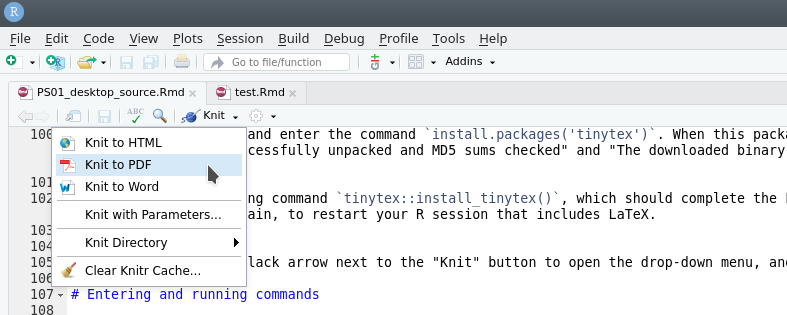
\includegraphics{figures/knit2pdf.png}

In a moment, you should see a PDF pop-up. If you don't see anything
pop-up, try looking in the folder where you saved the R Markdown
document.

\leavevmode\hypertarget{license}{}%
Note that if you want to knit to HTML again, you'll have to choose
``Knit to HTML'' in the drop-down menu again, rather than just pressing
the ``Knit'' button directly.

\hypertarget{entering-and-running-r-commands}{%
\section{Entering and running R
commands}\label{entering-and-running-r-commands}}

The code chunks are where you put R code in a R Markdown file. So far,
your ``knitted'' file (your output document file) doesn't show anything,
because we did not put any content in the code chunks yet!

Using your first code chunk, type the following command to create a new
variable called \texttt{x} with the value of 6.

\begin{Shaded}
\begin{Highlighting}[]
\NormalTok{x }\OtherTok{\textless{}{-}} \DecValTok{6}
\end{Highlighting}
\end{Shaded}

The arrow \texttt{\textless{}-} is called an \textbf{ASSIGNMENT
OPERATOR}, and tells R to save an object called \texttt{x} that has the
value of 6. This is similar to saving a value in a graphing calculator.

\begin{quote}
Note that whatever you want to save must always be to the left of the
assignment operator!!
\end{quote}

To actually \textbf{RUN} this command in your console, you have a few
options:

\begin{itemize}
\tightlist
\item
  click on the green triangle in the code chunk
\item
  highlight the code and hit \texttt{Control-Enter} on a PC or
  \texttt{Command-Return} on a Mac
\end{itemize}

Think of ``running'' code in your console as telling R ``do this''.

\leavevmode\hypertarget{license}{}%
Note that you now have a new object in your workspace, called x!

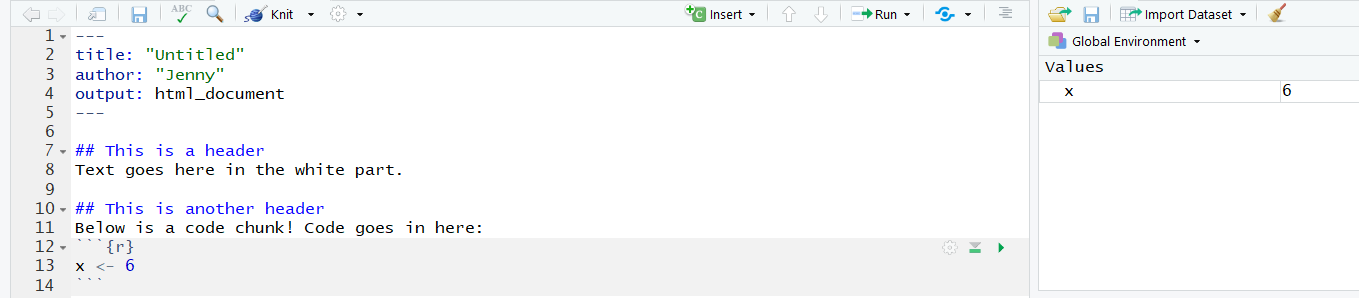
\includegraphics[width=1\textwidth,height=\textheight]{figures/workspacex.png}

\hypertarget{data-types--a-brief-intro}{%
\section{Data types- a brief intro}\label{data-types--a-brief-intro}}

So far you have made a numeric variable \texttt{x}. There many other
types of data objects you can make in R.

First, copy, paste and run the following command in a new code chunk to
make a \textbf{character} called \texttt{favorite\_movie}. Think of
characters as text as opposed to numerical values. Note that I told R
that this was a \textbf{character} by putting quotation marks around
\texttt{Star\_Wars}.

\begin{Shaded}
\begin{Highlighting}[]
\NormalTok{favorite\_movie }\OtherTok{\textless{}{-}} \StringTok{"Star\_Wars"}
\end{Highlighting}
\end{Shaded}

Next, copy, paste and run the following command into a new code chunk.

\begin{Shaded}
\begin{Highlighting}[]
\NormalTok{v }\OtherTok{\textless{}{-}} \FunctionTok{c}\NormalTok{(}\DecValTok{2}\NormalTok{, }\DecValTok{4}\NormalTok{, }\DecValTok{6}\NormalTok{)}
\end{Highlighting}
\end{Shaded}

This makes what is called a \textbf{vector}, which we have named
\texttt{v}. It is a data object that has multiple elements of the same
type. This vector contains three numbers, 2, 4, and 6. The \texttt{c()}
function says to r to \texttt{concatenate} the values 2, 4, 6, into a
single \textbf{vector}. Note in the Environment pane that your vector
\texttt{v} contains numbers (listed as \texttt{num}).

You can do math on a vector that contains numbers! For instance, copy,
paste and run the following command into a new code chunk. This tells R
to multiply each element of the vector \texttt{v} by 3.

\begin{Shaded}
\begin{Highlighting}[]
\NormalTok{v }\SpecialCharTok{*} \DecValTok{3}
\end{Highlighting}
\end{Shaded}

\hypertarget{practice-on-your-own}{%
\section{Practice on your own!}\label{practice-on-your-own}}

To complete this problem set you will next run through some Exercises,
and submit a knitted PDF file with answers all the Exercises. Please
make a \textbf{header} for each of these Exercises. If you need to
answer an Exercise with text, type the text \textbf{below} the header,
on the next line, in the white part, and if you need to answer an
Exercise with some code, insert a code chunk \textbf{below} the header,
and put the code in the greyed out box.

\leavevmode\hypertarget{license}{}%
Remember to save your work as you go along! Click the save button in the
upper left hand corner of the R Markdown window.

\begin{enumerate}
\def\labelenumi{\arabic{enumi}.}
\item
  Answer the following with code in a code chunk (no text necessary).
  Remember that the code is just \textbf{instructions} for R. You need
  to run the code chunk to make R execute those instructions!

  \begin{itemize}
  \tightlist
  \item
    Create a variable called \texttt{y} with the value of 7
  \item
    Multiply \texttt{x} by \texttt{y}, and store the answer in a
    variable named \texttt{z} like so: \texttt{z\ \textless{}-\ x\ *\ y}
  \item
    You should now see \texttt{favorite\_movie}, \texttt{x}, \texttt{v},
    \texttt{y}, and \texttt{z} all in your Environment pane
  \end{itemize}
\item
  \begin{itemize}
  \tightlist
  \item
    Run the following mathematical operation in a code chunk:
    \texttt{6\ +\ 3}
  \item
    Where does the answer appear? (please answer with \textbf{text})
  \end{itemize}
\item
  \begin{itemize}
  \tightlist
  \item
    Now add a code chunk, and save the results of \texttt{6\ +\ 3} as a
    variable called a.
  \item
    Does the answer appear? (please answer with \textbf{text})
  \item
    Where does the object \texttt{a} show up? (please answer with
    \textbf{text})
  \item
    Next type \texttt{a} into the code chunk and re-run the code chunk.
    What happens? (please answer with \textbf{text})
  \end{itemize}
\end{enumerate}

\leavevmode\hypertarget{license}{}%
It is a good idea to try kitting your document from time to time as you
go along! Go ahead, and make sure your document is knitting, and that
your PDF file includes Exercise headers, text, and code. Note that
knitting automatically saves your Rmd file too!

\begin{enumerate}
\def\labelenumi{\arabic{enumi}.}
\item
  \begin{itemize}
  \tightlist
  \item
    Run following command in a new code chunk. \texttt{a\^{}2}.
  \item
    What does the \texttt{\^{}} operator do? (please answer with
    \textbf{text})
  \end{itemize}
\item
  \begin{itemize}
  \tightlist
  \item
    Type the following command into a new code chunk.
    \texttt{sum(a,\ x,\ y)}
  \item
    \texttt{sum} is a function. Based on the output, what do you think
    the \texttt{sum} function does? (please answer with \textbf{text})
  \end{itemize}
\item
  \begin{itemize}
  \tightlist
  \item
    Click the little broom icon in the upper right hand corner of the
    \textbf{Environment} pane. Click yes on the window that opens.
  \item
    What happened? (please answer with \textbf{text}, and don't freak
    out)
  \end{itemize}
\item
  \begin{itemize}
  \tightlist
  \item
    Go to the \textbf{Run} button at the top right of the R Markdown
    pane, and choose \textbf{Run All} (the last option)
  \item
    What happened? (please answer with \textbf{text})
  \end{itemize}
\item
  Recall the vector \texttt{v} we created earlier. Copy, paste and run
  the following in a code chunk. What does this code accomplish? (please
  answer with \textbf{text})
\end{enumerate}

\begin{Shaded}
\begin{Highlighting}[]
\NormalTok{v }\SpecialCharTok{+} \DecValTok{2}
\end{Highlighting}
\end{Shaded}

\begin{enumerate}
\def\labelenumi{\arabic{enumi}.}
\tightlist
\item
  Copy, paste, and run the following code to make a vector called
  \texttt{music}, that contains music genres. Recall a vector is a data
  object that has multiple elements of the same type. Here the data type
  is a \textbf{character}. Look in the environment pane. How does R tell
  us that this vector contains \textbf{characters}, not numbers? (please
  answer with \textbf{text})
\end{enumerate}

\begin{Shaded}
\begin{Highlighting}[]
\NormalTok{music }\OtherTok{\textless{}{-}} \FunctionTok{c}\NormalTok{(}\StringTok{"bluegrass"}\NormalTok{, }\StringTok{"funk"}\NormalTok{, }\StringTok{"folk"}\NormalTok{)}
\end{Highlighting}
\end{Shaded}

\begin{enumerate}
\def\labelenumi{\arabic{enumi}.}
\tightlist
\item
  Now let's practice some basic formatting. Using this formatting tips
  page figure out how to put the following into your lab report. These
  all can get typed into the white section, where text goes.
  \textbf{Hint:} To put \textbf{each of these on its own line!} hit a
  hard return between each line of text!!!!!!!!
\end{enumerate}

\emph{Italicize like this}

\textbf{Bold like this}

A superscript: R\textsuperscript{2}

\begin{enumerate}
\def\labelenumi{\arabic{enumi}.}
\tightlist
\item
  \textbf{Extra credit:} What in the world does Charlie Brown have to do
  with R?
\end{enumerate}

\hypertarget{turning-in-your-work}{%
\section{Turning in your work}\label{turning-in-your-work}}

Each week you will submit a \textbf{PDF} file with all your code and
text on Gradscope. The steps to do this are as follows:

\begin{itemize}
\tightlist
\item
  Knit a final copy with all your changes and work, \textbf{making sure
  to choose ``Knit to PDF'' from the drop-down menu}.
\item
  Look at your final PDF file to make sure it contains the work you
  expect, and is formatted properly (e.g.~11-12 Exercise headers, each
  with answers for this week)
\item
  Locate the PDF file on your computer's hard drive. It should be found
  in the same folder as the R Markdown document where you did your work.
\item
  Upload the file to the corresponding assignment on Gradescope. If you
  haven't joined the couse on Gradesceope, click the ``Add Course''
  button on the home page after you login, and enter the enrollment code
  posted on the Moodle page.
\item
  In Gradescope, be sure to annotate the pages where your responses to
  each question are. You can find a helpful video on submitting an
  assignment on Gradescope
  \href{https://www.youtube.com/watch?v=KMPoby5g_nE}{here}.
\end{itemize}


\includegraphics[width=0.41\textwidth,height=\textheight]{figures/charlie_brown_1.jpg}
\includegraphics[width=0.17\textwidth,height=\textheight]{figures/charlie_brown_2.jpg}

\begin{center}\rule{0.5\linewidth}{0.5pt}\end{center}

\end{document}
